%%%%%%%%%%%%%%%%%%%%%%%%%%%%%%%%%%%%%%%%%%%%%%%%%%%%%%%%%%%%%%%%%%%%%%%%%%%%%%%%%%%%%
%																					%
%	TRABAJO: Proyecto Integrador													%
%																					%
%		Titulo: 	Desarrollo de IP cores con procesamiento de Redes de Petri 		%
%					Temporales para sistemas multicore en FPGA						%
%																					%
%		Autores:	Juli�n Nonino													%
%					Carlos Renzo Pisetta											%
%		Director:	Orlando Micolini												%
%																					%
%	Parte: Marco Teorico															%
%	Capitulo: FPGA - IP cores - HDL													%
%	Seccion: Field Programmable Gate Array											%	
%	Archivo: fpga.tex																%
%																					%
%%%%%%%%%%%%%%%%%%%%%%%%%%%%%%%%%%%%%%%%%%%%%%%%%%%%%%%%%%%%%%%%%%%%%%%%%%%%%%%%%%%%%

% Path Imagenes: ./marco_teorico/FPGA_IP_HDL/img
% Nombre predeterminado imagenes: fpgaxx
%	xx es el numero de imagen

\section{Field Programmable Gate Array}
	\label{sec:fpga}

	Una FPGA (Field Programmable Gate Array) es un circuito integrado digital formado por bloques
	l�gicos los interconectados.

	Las interconexiones de una FPGA pueden ser conFigurados mediante un Lenguaje de Descripci�n de 
	Hardware (HDL). De esta manera una FPGA puede reproducir desde simples compuertas l�gicas hasta 
	complejos sistemas dentro de un solo chip.

	Existen FPGAs que pueden ser reprogramadas lo que les permite una gran flexibilidad a la hora de
	dise�ar circuitos digitales. Por otro lado, existen FPGAs que solo pueden programarse una �nica 
	vez, su principal ventaja su menor consumo aunque al momento de dise�ar circuitos son mas complejas.

	En la \ref{fig:fpga01} se ve una FPGA dentro de una placa de desarrollo con diferentes perif�ricos ya 
	conectados.
	
	Las caracter�sticas f�sicas a tener en cuenta en la elecci�n de una FPGA depender�n del proyecto que se
	desea emprender, pero, principalmente se consideran los siguientes puntos:
	\begin{itemize}
	  \item \emph{Cantidad de bloques l�gicos}: determina el espacio disponible para implementar la l�gica.
	  \item \emph{Tipo y tama�o de memoria}: pudiendo ser \emph{distribuida} o \emph{de bloques}, donde existe una 
	  		memoria dedicada incluida en la FPGA o se utilizan los bloques l�gicos de la misma respectivamente.
	  \item \emph{Cantidad de puertos I/O}: usados como interface entre la FPGA y dispositivos externos.
	  \item \emph{Otros componentes internos}: Bloques de memoria, multiplicadores, PLL, CPU, conversores 
	  		A/D, bloques DSP, etc.
	\end{itemize}
	
	\begin{raggedright}
	Las FPGA ofrecen las siguientes ventajas:
	\end{raggedright}	
	\begin{itemize}
		\item Gran flexibilidad de producto.
		\item Posibilidad de actualizar tanto el firmware como el hardware.
		\item Reutilizaci�n del hardware.
		\item Son dispositivos reconFigurables.
		\item Bajo costo respecto a los ASIC.
		\item Ejecuci�n de circuitos m�s r�pida que en otros dispositivos reprogramables.
		\item \textbf{La ejecuci�n de cada bloque se realiza concurrentemente, a diferencia de un micro controlador.}
		\item Gran utilidad para dise�o y testing de prototipos. 
	\end{itemize}
	\begin{raggedright}
		Por otro lado, tienen las siguientes desventajas:
	\end{raggedright}
	\begin{itemize}
		\item M�s costosas que los microprocesadores equivalentes.
		\item Mayor complejidad de dise�o (soft+hard).
		\item Retardos de propagaci�n mayores a los existentes en ASIC (Application Specific Integrated Circuit).
		\item Mayores costos en producci�n a gran escala.
		\item Consumo est�tico y din�mico moderados.
	\end{itemize}	
	\begin{figure}[H]
		\centering
		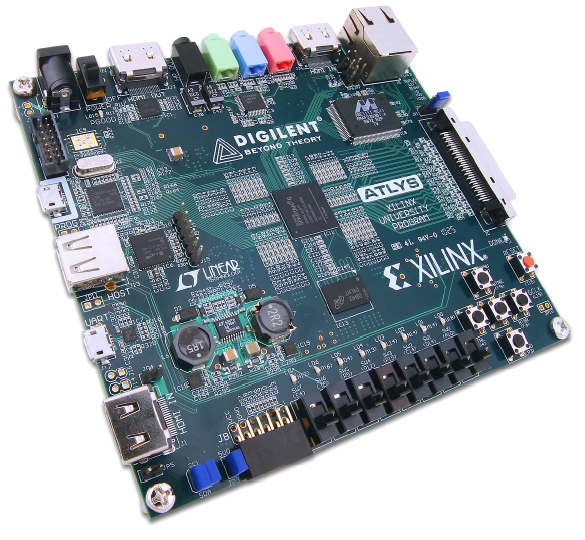
\includegraphics[width=.4\linewidth]{./marco_teorico/FPGA_IP_HDL/img/fpga01}
		\caption{Atlys Spartan-6 FPGA Development Board}
		\label{fig:fpga01}
	\end{figure}
	\newpage